\documentclass{article}

% Packages
\usepackage{amsmath} % AMSmath
\usepackage[skip=10pt plus1pt, indent=0pt]{parskip} % Manage paragraph spacing

\usepackage{subcaption} % Subfigures and subtables
\usepackage[aboveskip=1pt,skip=3pt,labelfont=bf,labelsep=period,justification=raggedright,singlelinecheck=off]{caption} % Manage table and figure captions
\usepackage{todonotes} % Pop-up "to do" notes


% Hyperlink management
\usepackage[hypertexnames=false]{hyperref} 
\hypersetup{colorlinks=true, citecolor = black, linkcolor=black, filecolor=magenta, urlcolor=black} % Hyperlink style options

% Cleveref must be loaded after hyperref
\usepackage[capitalise]{cleveref}

% For numbering just one line of an equation
\newcommand\numberthis{\addtocounter{equation}{1}\tag{\theequation}}


% Tikz
\usepackage{tikz} % Tikz
\usetikzlibrary{arrows.meta} % Tikz arrows
\tikzset{nodes={font=\sffamily}} % Tikz custom font

% Shorthand
\DeclareMathOperator{\dee}{d\!} % Derivative "d"
% \newcommand{\etall}{\emph{et. al }} % Nice "et. al" % Shouldn't need, use \citet instead.

% Colours
\definecolor{c1}{HTML}{A53F2B} % Red
\definecolor{c2}{HTML}{AD6A36} % Orange
\definecolor{c3}{HTML}{B59441} % Beige
\definecolor{c4}{HTML}{887D3D} % Light green
\definecolor{c5}{HTML}{5A6638} % Dark green\\

\usetikzlibrary{external}
\tikzexternalize % activate!

\begin{document}

% No control model

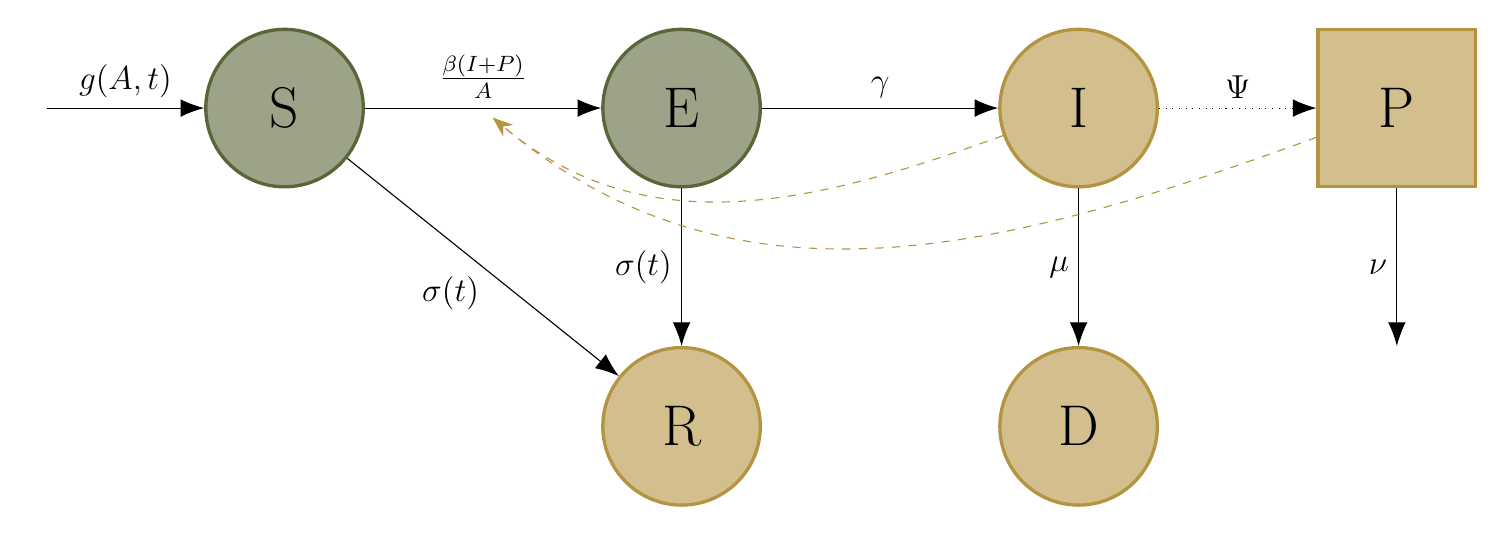
\begin{tikzpicture}[
%Set node styles
n1/.style={circle, draw=c3, fill=c3!60, very thick, minimum size=2cm},
n2/.style={circle, draw=c5, fill=c5!60, very thick, minimum size=2cm},
n3/.style={rectangle, draw=c3, fill=c3!60, very thick, minimum size=2cm}
]

% Draw nodes
\node(preS){};
\node[n2](S)[right= 2cm of preS]{\huge $\mathrm{S}$};
\node[n2](E)[right= 3cm of S]{\huge $\mathrm{E}$};
\node[n1](I)[right= 3cm of E]{\huge $\mathrm{I}$};
\node[n1](R)[below= 2cm of E]{\huge $\mathrm{R}$};
\node[n1](D)[below= 2cm of I]{\huge $\mathrm{D}$};
\node[n3](P)[right= 2cm of I]{\huge $\mathrm{P}$};
\node(Pout)[below= 2cm of P]{};

% Draw progression arrows
\draw[-{Latex[length=3mm]}] (preS) -- (S) node[midway, above]{\large $g(A,t)$};
\draw[-{Latex[length=3mm]}] (S) -- (E) node[midway, above]{\large $ \frac{\beta(I+P)}{A}$};
\draw[-{Latex[length=3mm]}] (E) -- (I) node[midway, above]{\large $\gamma$};
\draw[-{Latex[length=3mm]}] (P) -- (Pout) node[midway, left]{\large $\nu$};
\draw[dotted, -{Latex[length=3mm]}] (I) -- (P) node[midway, above]{\large $\Psi$};
\draw[-{Latex[length=3mm]}] (S) -- (R) node[midway, below]{\large $\sigma(t) \qquad$};
\draw[-{Latex[length=3mm]}] (E) -- (R) node[midway, left]{\large $\sigma(t)$};
\draw[-{Latex[length=3mm]}] (I) -- (D) node[midway, left]{\large $\quad \mu$};

% Draw infection arrows
\node(SEarrow)[right= 1.5cm of S]{};
\draw[c3, dashed, -{Stealth[length=2.5mm]}] (P) to [out = 200, in = -40] (SEarrow.south);
\draw[c3, dashed, -{Stealth[length=2.5mm]}] (I) to [out = 200, in = -40] (SEarrow.south);

\end{tikzpicture}





% Cross contact model
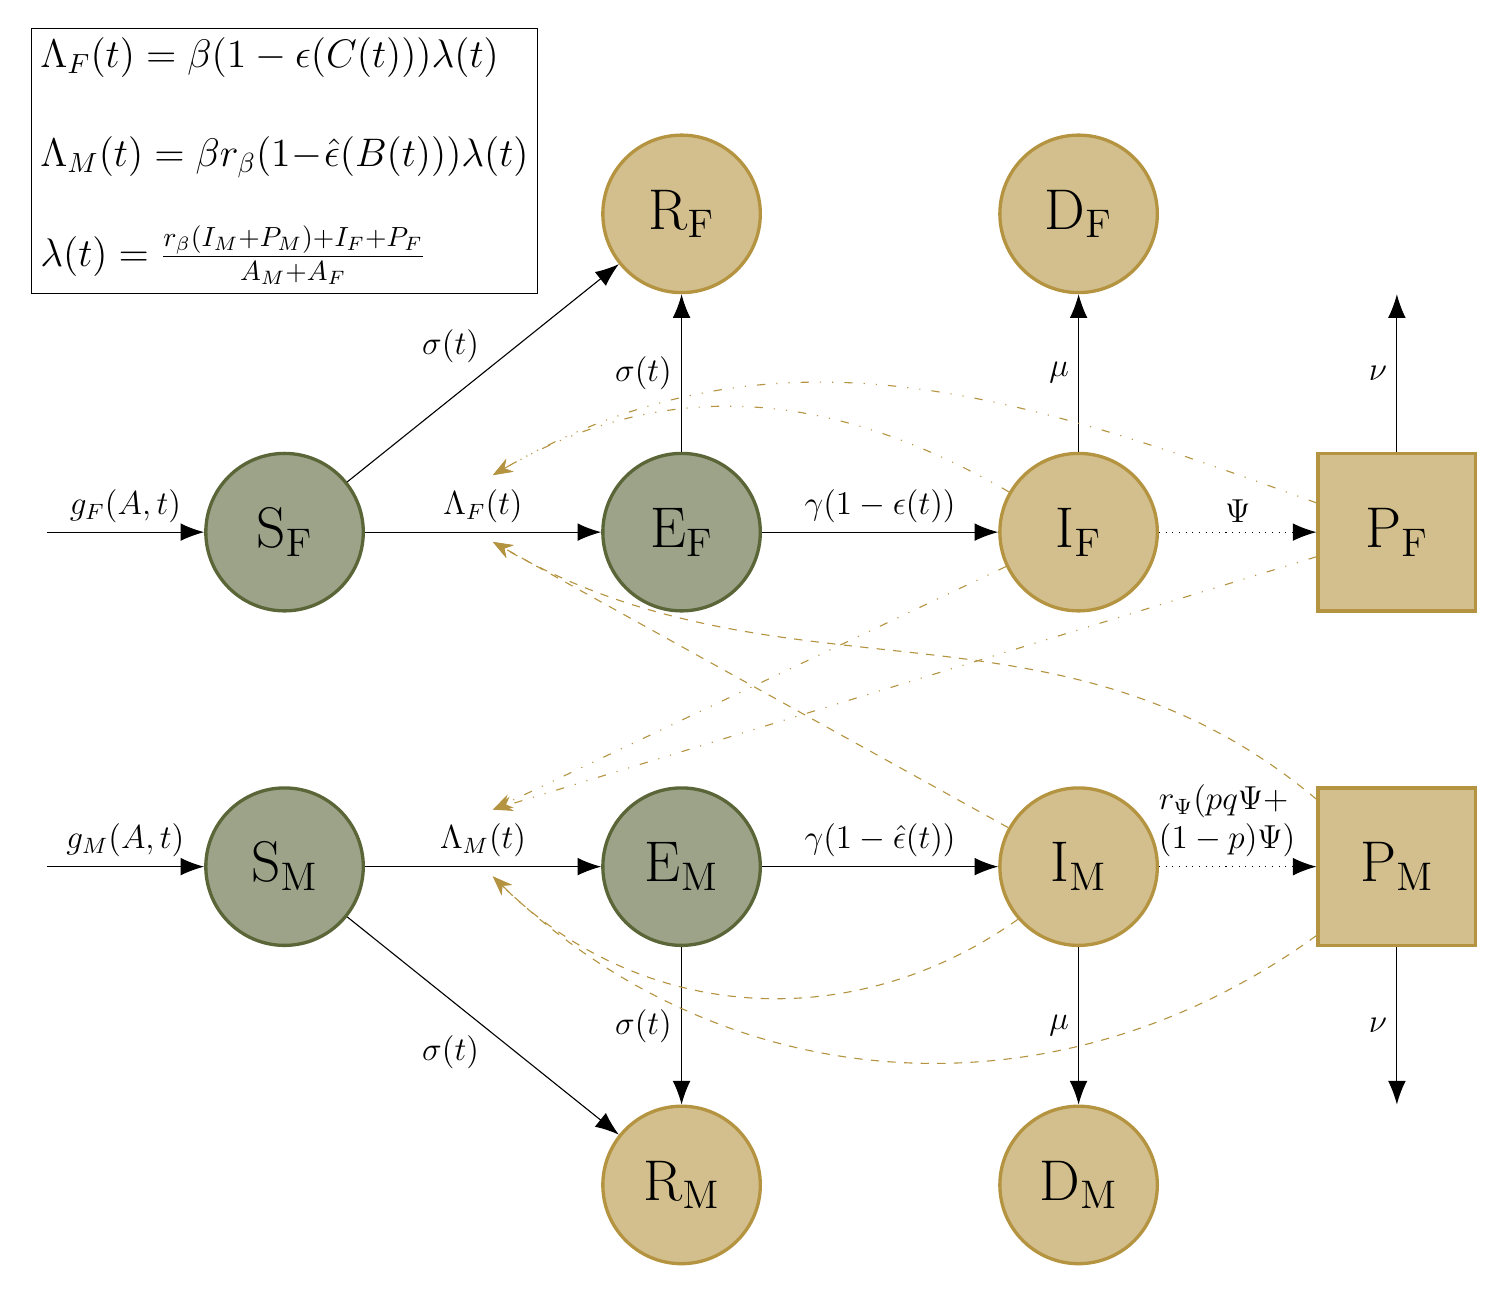
\begin{tikzpicture}[
%Set node styles
n1/.style={circle, draw=c3, fill=c3!60, very thick, minimum size=2cm},
n2/.style={circle, draw=c5, fill=c5!60, very thick, minimum size=2cm},
n3/.style={rectangle, draw=c3, fill=c3!60, very thick, minimum size=2cm},
n4/.style={rectangle, draw=black, fill=white}
]

% Fungicide
% Draw nodes
\node(preSF){};
\node[n2](SF)[right= 2cm of preSF]{\huge $\mathrm{S_F}$};
\node[n2](EF)[right= 3cm of SF]{\huge $\mathrm{E_F}$};
\node[n1](IF)[right= 3cm of EF]{\huge $\mathrm{I_F}$};
\node[n1](RF)[above= 2cm of EF]{\huge $\mathrm{R_F}$};
\node[n1](DF)[above= 2cm of IF]{\huge $\mathrm{D_F}$};
\node[n3](PF)[right= 2cm of IF]{\huge $\mathrm{P_F}$};
\node(PoutF)[above= 2cm of PF]{};

% Draw progression arrows
\draw[-{Latex[length=3mm]}] (preSF) -- (SF) node[midway, above]{\large $g_F(A,t)$};
\draw[-{Latex[length=3mm]}] (SF) -- (EF) node[midway, above]{\large $\Lambda_F(t)$};
\draw[-{Latex[length=3mm]}] (EF) -- (IF) node[midway, above]{\large $\gamma(1-\epsilon(t))$};
\draw[-{Latex[length=3mm]}] (PF) -- (PoutF) node[midway, left]{\large $\nu$};
\draw[dotted, -{Latex[length=3mm]}] (IF) -- (PF) node[midway, above]{\large $\Psi$};
\draw[-{Latex[length=3mm]}] (SF) -- (RF) node[midway, above]{\large $\sigma(t) \qquad$};
\draw[-{Latex[length=3mm]}] (EF) -- (RF) node[midway, left]{\large $\sigma(t)$};
\draw[-{Latex[length=3mm]}] (IF) -- (DF) node[midway, left]{\large $\quad \mu$};

% Draw infection arrows
\node(SEinterF)[right= 1.5cm of SF]{};
\node(SEarrowF)[above= 0.6cm of SEinterF]{};
\draw[c3, loosely dash dot dot, -{Stealth[length=2.5mm]}] (PF) to [out = 160, in = 30] (SEarrowF.south);
\draw[c3, loosely dash dot dot, -{Stealth[length=2.5mm]}] (IF) to [out = 150, in = 30] (SEarrowF.south);



% IPM
% Draw nodes
\node(preSM)[below= 4cm of preSF]{};
\node[n2](SM)[right= 2cm of preSM]{\huge $\mathrm{S_M}$};
\node[n2](EM)[right= 3cm of SM]{\huge $\mathrm{E_M}$};
\node[n1](IM)[right= 3cm of EM]{\huge $\mathrm{I_M}$};
\node[n1](RM)[below= 2cm of EM]{\huge $\mathrm{R_M}$};
\node[n1](DM)[below= 2cm of IM]{\huge $\mathrm{D_M}$};
\node[n3](PM)[right= 2cm of IM]{\huge $\mathrm{P_M}$};
\node(PoutM)[below= 2cm of PM]{};

% Draw progression arrows
\draw[-{Latex[length=3mm]}] (preSM) -- (SM) node[midway, above]{\large $g_M(A,t)$};
\draw[-{Latex[length=3mm]}] (SM) -- (EM) node[midway, above]{\large $\Lambda_M(t)$};
\draw[-{Latex[length=3mm]}] (EM) -- (IM) node[midway, above]{\large $\gamma(1-\hat{\epsilon}(t))$};
\draw[-{Latex[length=3mm]}] (PM) -- (PoutM) node[midway, left]{\large $\nu$};
\draw[dotted, -{Latex[length=3mm]}] (IM) -- (PM) node[midway, above] {\large \parbox{2cm}{$r_\Psi(pq\Psi +$ \\  $(1-p)\Psi)$}};
\draw[-{Latex[length=3mm]}] (SM) -- (RM) node[midway, below]{\large $\sigma(t) \qquad$};
\draw[-{Latex[length=3mm]}] (EM) -- (RM) node[midway, left]{\large $\sigma(t)$};
\draw[-{Latex[length=3mm]}] (IM) -- (DM) node[midway, left]{\large $\quad \mu$};

% Draw infection arrows
\node(SEarrowM)[right= 1.5cm of SM]{};
\node(SEinterM)[above= 0.6cm of SEarrowM]{};
\draw[c3, dashed, -{Stealth[length=2.5mm]}, bend right=-40, text=c4] (PM) to node[midway, above]{} (SEarrowM.south);
\draw[c3, dashed, -{Stealth[length=2.5mm]}, bend right=-40, text=c4] (IM) to node[midway, above]{} (SEarrowM.south) ;



% Cross field contact
% Draw infection arrows
% M -> F
\draw[c3, dashed, -{Stealth[length=2.5mm]}, text=c4] (PM) to [out = 140, in = -30] (SEinterF.south);
\draw[c3, dashed, -{Stealth[length=2.5mm]}, text=c4] (IM) to (SEinterF.south) ;
\node(infection1)[above right=2.1cm of IM, text=c4]{};
\node(infection2)[above left=0.3cm of IM, text=c4]{};

% F -> M
\draw[c3, loosely dash dot dot, -{Stealth[length=2.5mm]}, text=c4] (PF) to (SEinterM.south);
\draw[c3, loosely dash dot dot, -{Stealth[length=2.5mm]}, text=c4] (IF) to (SEinterM.south) ;

% Put in legend
\node[n4](legend)[above = 2cm of SF]{\Large \parbox{6.2cm}{$\Lambda_F(t) = \beta (1-\epsilon(C(t))) \lambda(t)$ \\  \\ $\Lambda_M(t) = \beta r_\beta (1-\hat{\epsilon}(B(t)))\lambda(t)$ \\ \\ $\lambda(t) = \frac{r_\beta (I_M + P_M) + I_F + P_F}{A_M + A_F}$}}{};

\end{tikzpicture}

\end{document}\\
